\chapter[Amino acid and protein encoding]{Hyperdimensional computing methods to encode amino acids and protein sequences}
\section{Introduction}
To research the possibilities of the hyperdimensional computing framework applied to protein language modeling, we introduce a rudimentary pipeline. First, amino acids have to be encoded into hyperdimensional vectors. Second, these vectors for every separate amino acid can be then further encoded into vectors representing a full protein sequence. And lastly, these embeddings could be then utilized to perform predictions such as classifications as shown in Figure~\ref{fig:pipeline}. The first two steps of this pipeline will be discussed further in this chapter.

\begin{figure}[H]
    \centering
    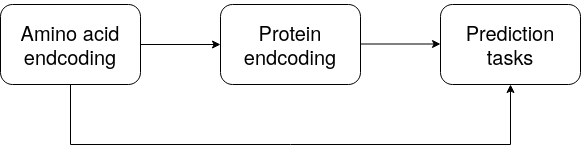
\includegraphics[scale = 0.5]{pipeline}
    \caption{A simple demonstration of the proposed workflow. First, we encode individual amino acids into hyperdimensional vectors. With these, protein sequences could be encoded into hyperdimensional vectors. Lastly, both kinds of embeddings could be then used for prediction tasks.}\label{fig:pipeline}
\end{figure}

\section{Encoding single amino acids into hyperdimensional vectors}
Currently, in most of the research in hyperdimensional computing, there is an emphasis on creating and assigning hyperdimensional vectors to certain concepts at random. This is useful for optimizing speed and efficiency and is not a problem for many prevalent research areas such as natural language processing, where, for example, it is typically assumed that a letter's similarity to other letters in the alphabet remains constant. However, the practical application of hyperdimensional computing to biological data remains limited at present, posing a challenge in extending its utility to this specific domain. Some notable studies include HDNA which assigns random hyperdimensional vectors to DNA bases to encode DNA sequences and BioHD~\cite{biohd} which encodes protein sequences using random mRNA hypervectors to use in genome sequence searches. In the context of DNA sequencing, the assumption of assigning random hyperdimensional vectors may not present as significant an issue as with proteins. This is largely due to the distinct nature of DNA bases as they do not display the same degree of physicochemical diversity that amino acids in proteins do. DNA bases serve primarily as the information carrier in the biological system, with their sequence dictating the sequence of amino acids in proteins. In this role, the relevance of their physicochemical properties to their informational role is rather limited in comparison to amino acids, which main function is to dictate the structure and function of the resulting protein. Whilst there are phenomena in DNA structures such as base stacking and hydrogen bonding that play a role, the simple base-to-vector mapping often suffices.

When considering protein language modeling, however, this assumption might be suboptimal since some amino acids are chemically more similar to each other than to others which is crucial to the protein's structure and function. We can already estimate physicochemical distances between amino acids based on their physicochemical properties~\cite{physicochem} such as volume, polarity, chemical groups etc.\ \textit{via} many kinds of distance measures. The differing similarities between amino acids are tied into the structure and thus function of amino acid sequences and shape our view of protein language. It explains why some amino acid substitutions can result in almost no phenotypical changes or on the other hand detrimental changes. Proteins have evolved to maintain their structure and function, and drastic changes in physicochemical properties can disrupt these characteristics. Therefore, amino acid substitutions that preserve the physicochemical properties of the original amino acid are more likely to be selected, resulting in a negative correlation with physicochemical distance. To account for this, we experimented with several methods to encode physicochemical distance into amino acid hypervectors.

Besides encoding amino acids as building blocks, it is also useful to encode amino acids in the context they are found in. State-of-the-art protein language models have the ability to gather information on long-range dependencies around a single amino acid and encode this information into neural networks and in dense numerical vectors. These models are very powerful, but, as discussed earlier, very resource-intensive as well. To investigate the possibilities of developing contextual embeddings at the level of amino acids, we propose a novel encoding technique within the hyperdimensional computing framework.

\section{Encoding proteins into hyperdimensional vectors}
Once hyperdimensional vectors are constructed for each amino acid, the next step is to combine these vectors to form representations of protein sequences. We can draw inspiration from the operations in hyperdimensional computing, which have already been applied in natural language processing. Similar to how characters are combined to form words and sentences, we can leverage similar principles to combine amino acids and generate meaningful representations of protein sequences.

In Section~\ref{ssec:protclas}, we introduced the bag-of-words (BoW) method of embedding sequences in hyperdimensional space, which has been extensively applied to cases related to natural language processing in a hyperdimensional computing context. We also introduce a novel sequence embedding method in hyperdimensional computing.

\section{Methods}
From here on, every hyperdimensional vector is made to be 10,000-dimensional with randomly assigned binary elements unless noted otherwise. 
\subsection{Encoding single amino acids into hyperdimensional vectors}
\subsubsection*{Projected ESM-2 embeddings}
The last layer of the 3 billion-parameter ESM-2 model~\cite{esm2} of every amino acid was extracted, resulting in a 1024-dimensional real-valued embedding for every amino acid. To project these into hyperdimensions, a simple matrix multiplication has been employed: \[A \times B = C\],
where $A$ is a 1024-dimensional ESM-2 embedding and $B$ a matrix of 1024 random 10,000-D vectors. The resulting vectors are then min-max scaled and rounded depending on the desired nature of the vectors. To visually assess these, the vectors for each amino acid are reduced in dimensiond \textit{via} PCA into two dimensions. This has been compared to a PCA of the unaltered 1024-dimensional ESM-2 embeddings.
\subsubsection*{Real-valued projected ESM-2 embeddings}
It is possible to step away from binary hyperdimensional vectors, which are typically used in hyperdimensional computing research, and allow the vectors to be real-valued. This gives us the possibility to store more data in a vector and utilize more complex mathematical operations at the cost of losing the efficiency of bit-operations. We generated random real-valued vectors with random values in [-1,1]. Real-valued ESM-2 embeddings were generated by the same procedure as above, but without the rounding.
\subsubsection*{Enforcing similarities using genetic algorthims}
Instead of utilizing embeddings coming from other large protein language models, we also experimented with encoding predetermined target pairwise distances onto initially random hyperdimensional vectors. First, a suitable matrix with predetermined pairwise distances has to be considered. This also implies that the matrix has to be symmetric. If we then consider the 20 essential amino acids, the problem at hand would involve a set of 20 binary vectors of length 10,000 to conform to a target distance matrix based on Hamming distance. This can be classified as a combinatorial optimization problem as it involves searching for an optimal or near-optimal configuration of binary vectors that satisfy a specific criterion. To minimize the difference between the target and actual Hamming distances for all pairs of binary vectors, we could adjust the vectors by randomly bit-flipping them until they meet the desired criteria. However, the search space in this problem is vast ($2^{10,000 x 20}$), making exhaustive search methods computationally infeasible. Thus, more efficient algorithms are needed to solve this problem such as genetic algorithms~\cite{GA} (GAs). GAs, a subfield of evolutionary algorithms, draw inspiration from the process of natural selection and emulate the evolutionary mechanisms of crossover, mutation, and selection to explore a vast search space and converge toward an optimal or near-optimal solution. A genetic algorithm was implemented with the Evolutionary.jl package~\cite{evojl} in Julia to encode target similarities. The primary steps of a genetic algorithm include:
\begin{itemize}
    \item Initialization: random candidate solutions are initiated with a given population size.
    \item Crossover: Combine genetic material offspring of two parents (in this case vectors). There are many recombination techniques such as single-point, multi-point and uniform crossover.
    \item Mutation: Randomly alter genes (in this case bits) to explore other possibilities of configurations and prevent premature convergence due to local optima.
    \item Evaluation: Each individual in the population (in this case a set of vectors) is assessed using a fitness function, which measures how well the solution solves the given problem.
    \item Selection: Individuals from the population are selected based on their fitness to create a mating pool. Fitter individuals have a higher probability of being selected, mimicking the concept of survival of the fittest in natural evolution.
\end{itemize}
These steps are reiterated over a number of generations to obtain a set of vectors that correspond to the best fitness. A BLOSUM62 substitution matrix \cite{blosum} and Grantham's distance matrix \cite{aa_evolution} were considered as target pairwise similarity matrices for the GA. These were then normalized to obtain the target pairwise Hamming distances. The fitness is determined by the sum of the squared differences between the computed distance matrix of an individual and the target distance matrix. The lower the fitness value, the more optimal the individual. The population size was set to 25,000 and the number of generations to 250. The mutation rate was set to 0.15 and the crossover rate to 0.2; these are high and low respectively compared to more commonly used parameters because we want to emphasize the bit-flipping and avoid recombination of vectors for faster convergence.
\subsubsection*{Contextualized neighborhood-encoding of amino acids}\label{sssec:trans}
To encode the neighborhood of an amino acid in a sequence, all possible pairwise interactions with the central amino acid in question in a given window are made \textit{via} binding and then all encoded into one vector \textit{via} bundling as shown Figure~\ref{fig:AAtr}. Our neighborhood-encoder was tested on the human reference proteome in UniProt, entry \textit{UP000005640}, containing 20591 proteins. We started with real-valued random vectors and real-valued projected ESM-2 vectors for every amino acid. Windows of $n = 4$ and $n = 50$ were considered resulting in four different experiments. Every single residue in the human reference proteome was encoded with information within the $n$-range window and an average vector was made for every amino acid. For all 20591 peptides in the reference proteome, this procedure took only three hours for $n = 4$, but upwards to 15 hours for $n = 50$ on a high-performance computing cluster (HPC). After all amino acids were encoded, an element-wise average was made for every amino acid. The resulting hyperdimensional vectors were kept to a real-valued nature to not lose information for illustrative purposes. Principal component analysis was then done for these four experiments as seen in Figure~\ref{fig:bigfig}. 

\begin{figure}[ht!]
    \centering
    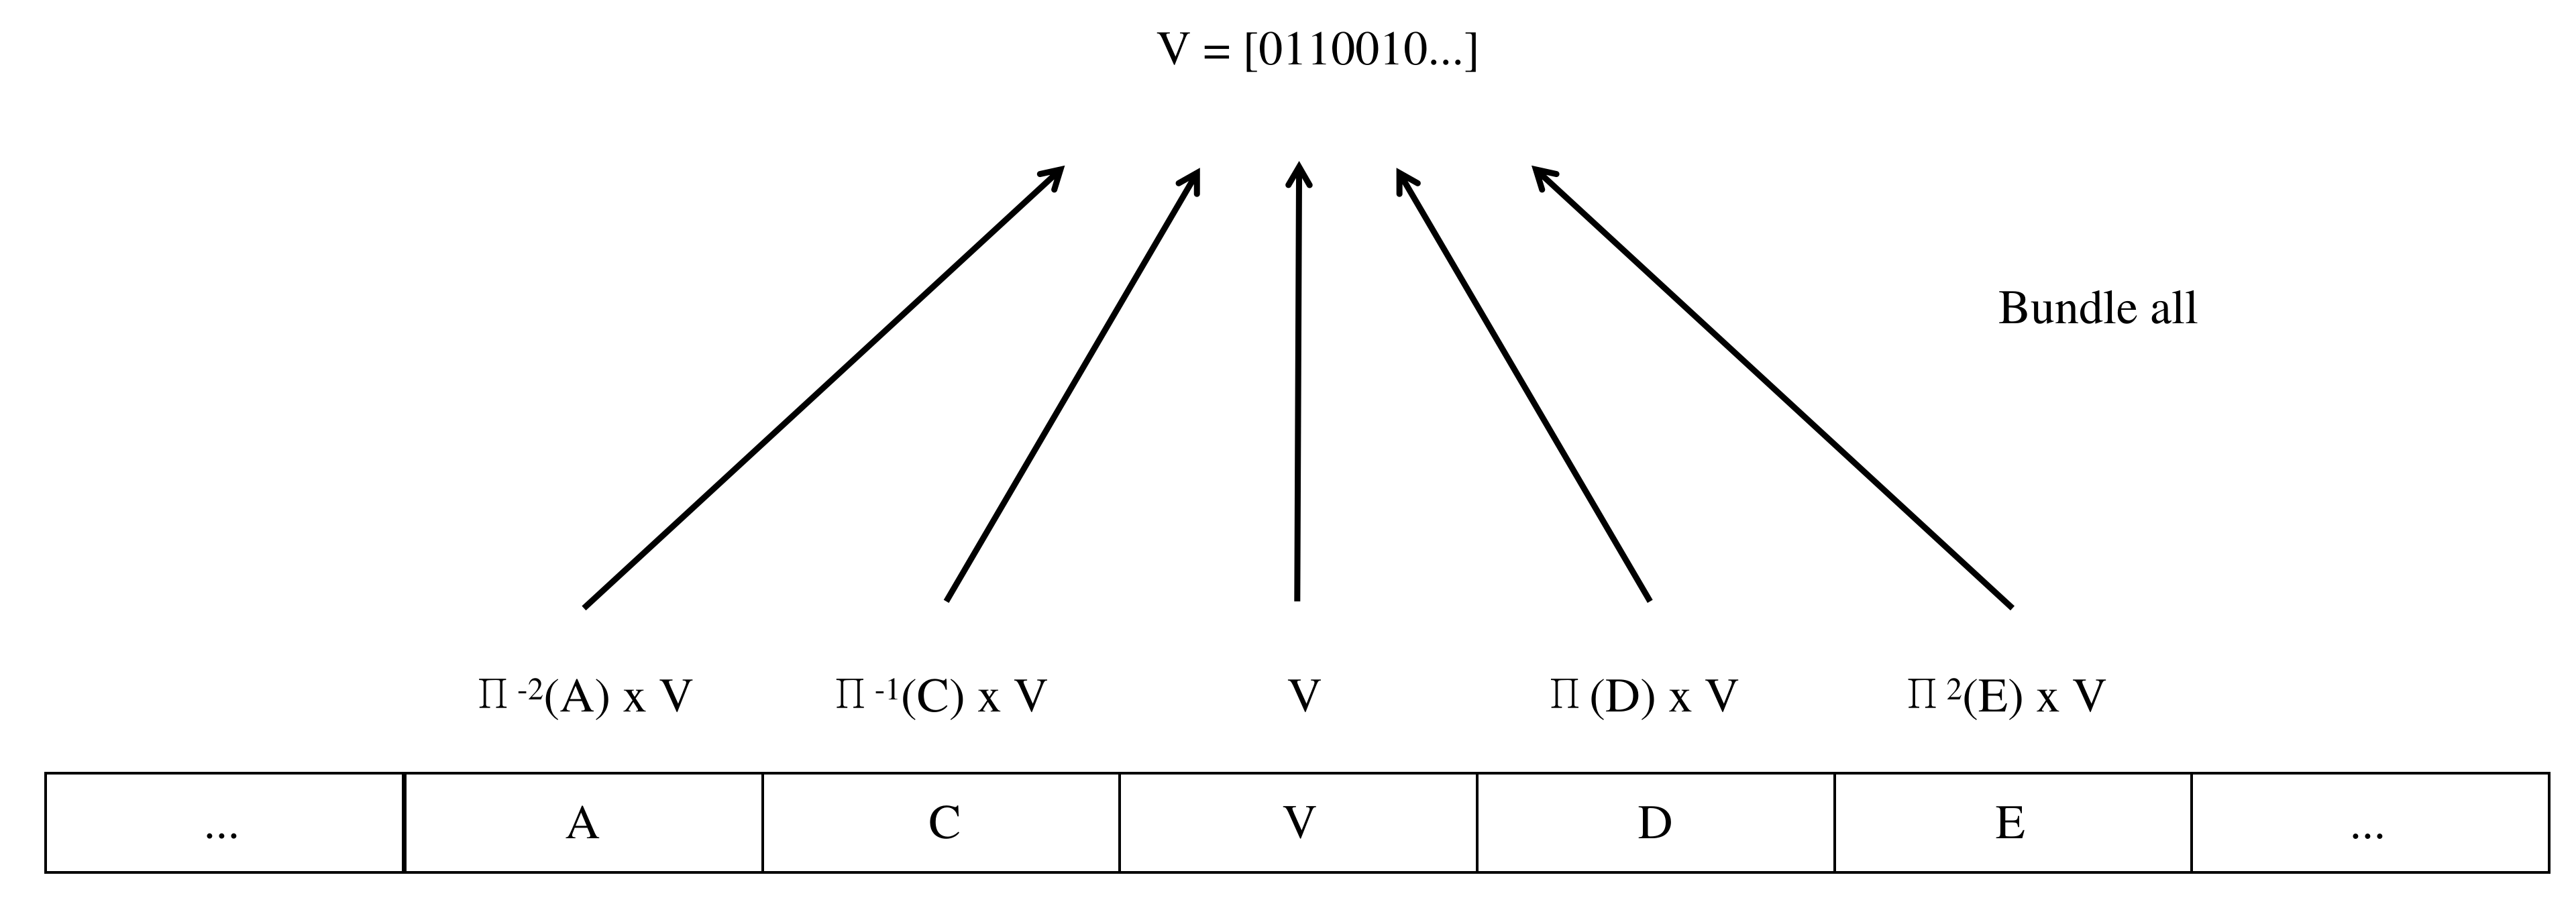
\includegraphics[scale = 0.43]{transformerlike}
    \caption{A simple demonstration of our amino acid encoder. First, HDVs are generated for every kind of amino acid, this can be done using just random HDVs, projected ESM-2 embeddings, GA-optimized vectors, etc. It considers an amino acid and all amino acids in a predetermined neighborhood (here $n = 2$). It produces all possible interactions of the central amino acid in the window by binding and then bundles all the pairwise interactions into one hyperdimensional vector that represents the central amino acid.}\label{fig:AAtr}
\end{figure}

\subsection{Encoding proteins into hyperdimensional vectors}\label{ssec:protseq}
We implemented two different algorithms to encode amino acid vectors into vectors representing proteins. We already introduced the BoW-method in Section~\ref{ssec:protclas}, fully explained in Figure~\ref{fig:diagram_exprot5}. We also introduce a novel sequence embedding method in hyperdimensional computing.  It is similar to the bag-of-words method in the sense that it bundles vectors of $k$-mers, but here, the $k$-mer's positional information will be encoded into the $k$-mer by permuting it before bundling as seen in Figure~\ref{fig:cnn}, similarly to how a convolutional layer in a neural network operates so we will name it the convolutional embedding method from here on. These methods will be extensively utilized and tested in Chapters 4 and 5 where several case studies consisting of protein sequences datasets are tackled.

\begin{figure}[ht!]
    \centering
    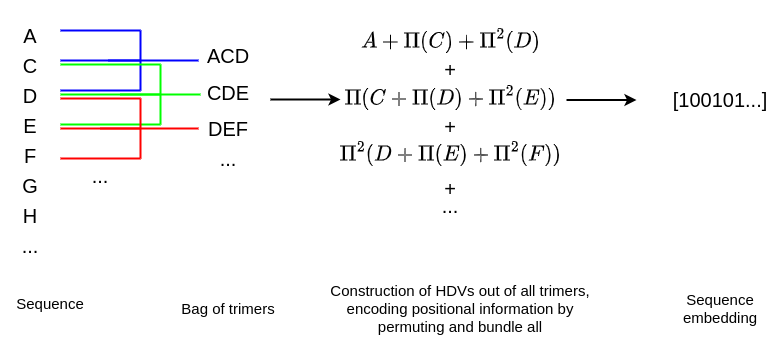
\includegraphics[scale = 0.6]{cnn.png}
    \caption{Overview of operations done to obtain an HDV from a sequence using the convolutional embedding method. First, an HDV is generated for every amino acid. Next, a peptide sequence is to be considered as a bag of trimers. A vector representing a trimer is generated by binding the three amino acids whilst retaining sequential information by shifting as in Eq.~\ref{eqn:trimer}, just as in the BoW-method (Figure~\ref{fig:diagram_exprot}). On top of that, every trimer will also be positionally encoded via a permutation operation. All retrievable trimers from a given sequence are then bundled together, forming a hyperdimensional vector representative of the sequence.}\label{fig:cnn}
\end{figure}

\section{Results}
\subsection{Projected ESM-2 embeddings}
Visually, no interesting patterns can be deducted from the PCA decompositions of the ESM-2 embeddings. Yet, if we also perform a principal component analysis on random vectors, we can see there is significantly more variance encoded into the first two principal components of the ESM embeddings (22 \%) compared to random vectors (10.5 \%, can deviate slightly depending on the run), meaning that there should be a significant amount of similarity encoded into the hyperdimensional vectors. PCA decomposition of our projected ESM-2 embeddings can't fully retrieve the variance in the hyperdimensional vectors as well as in the unaltered ESM-2 embeddings, as to be expected. The performance and usefulness may be shown more clearly when tested in other computational biology problem settings.

\begin{figure}[H]
\centering
\begin{minipage}[b]{.5\textwidth}
    \begin{subfigure}[b]{\textwidth}
    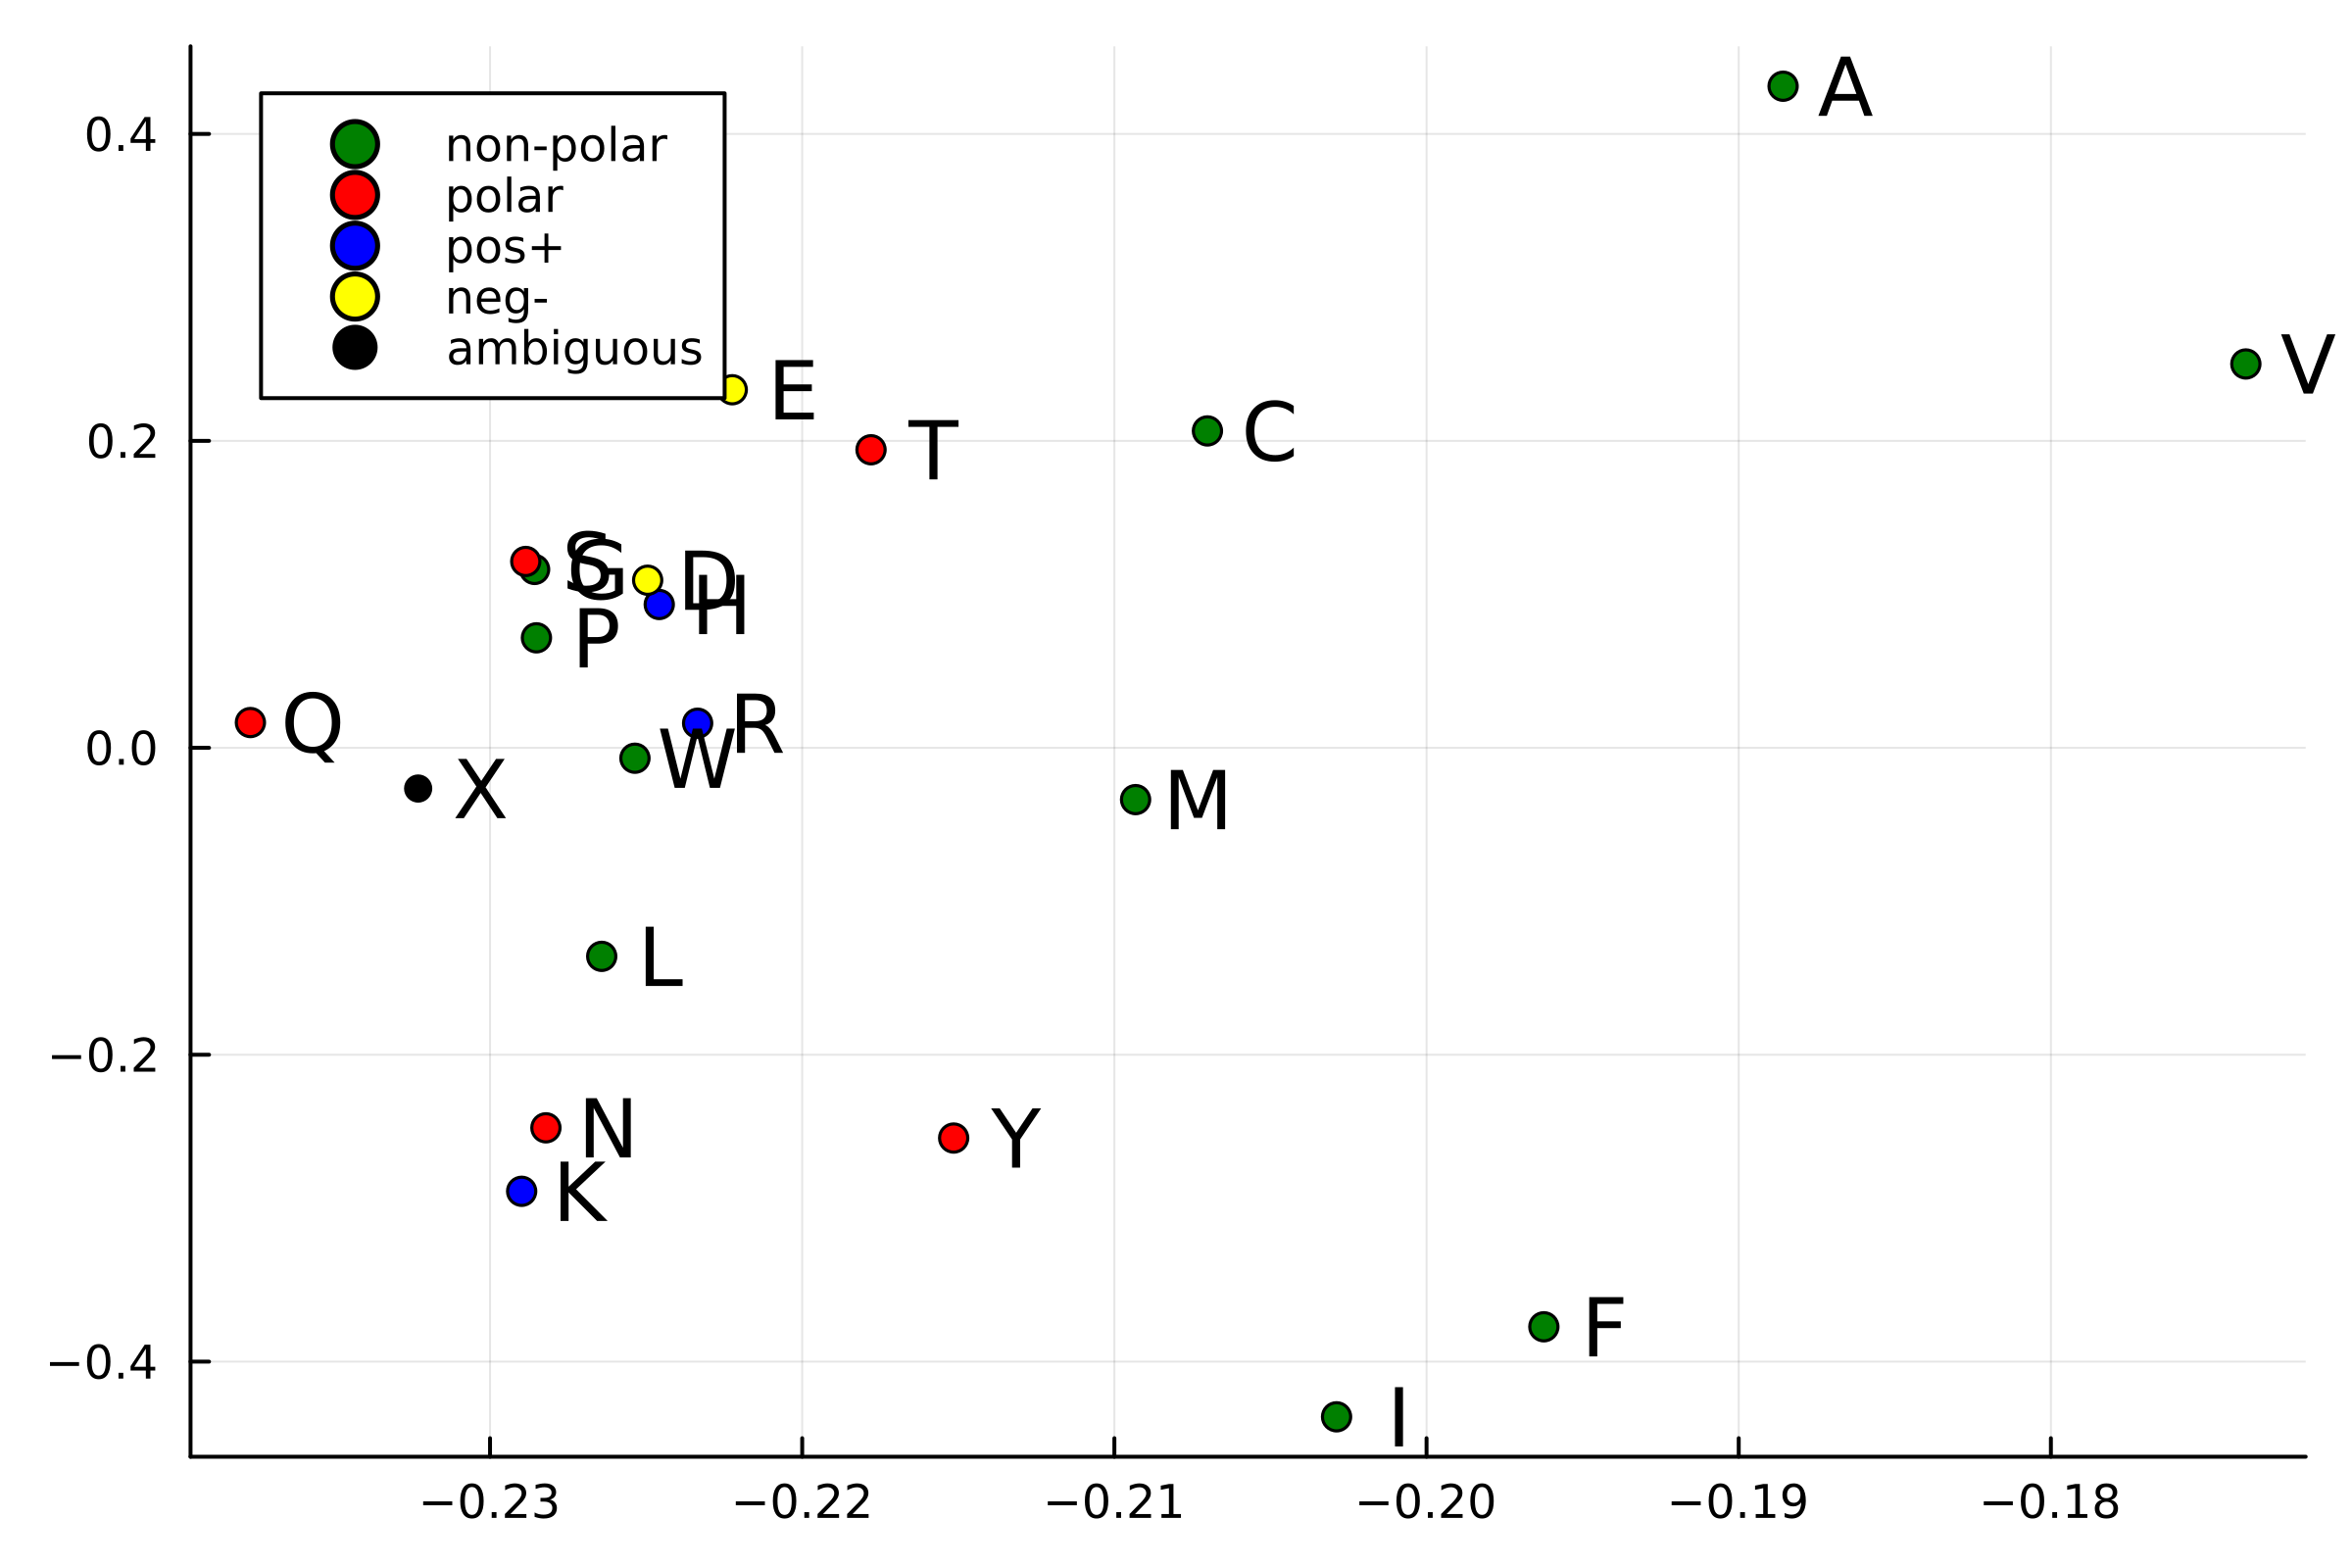
\includegraphics[width=\textwidth]{esm_emb_1028}
    \caption{Unaltered 1024-dimensional ESM-2 embeddings}
    \label{fig:AAesm_pure}
\end{subfigure}
\end{minipage}
\\
\centering
\begin{minipage}[b]{.5\textwidth}
\begin{subfigure}[b]{\textwidth}
    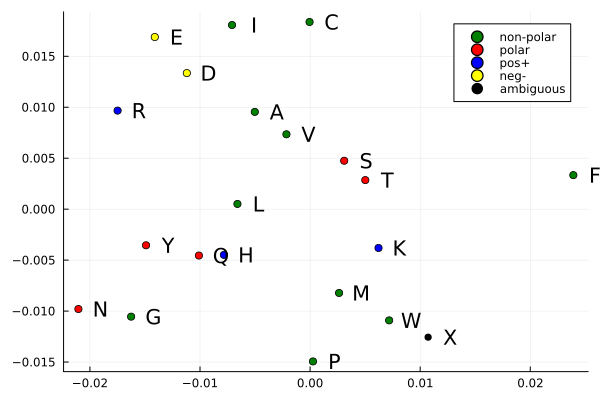
\includegraphics[width=\textwidth]{esm_emb}
    \caption{ESM-2 embeddings projected into binary hyperdimensionality}
    \label{fig:AAesm}
\end{subfigure}
\end{minipage}
\\
\centering
\begin{minipage}[b]{.5\textwidth}
\begin{subfigure}[b]{\textwidth}
    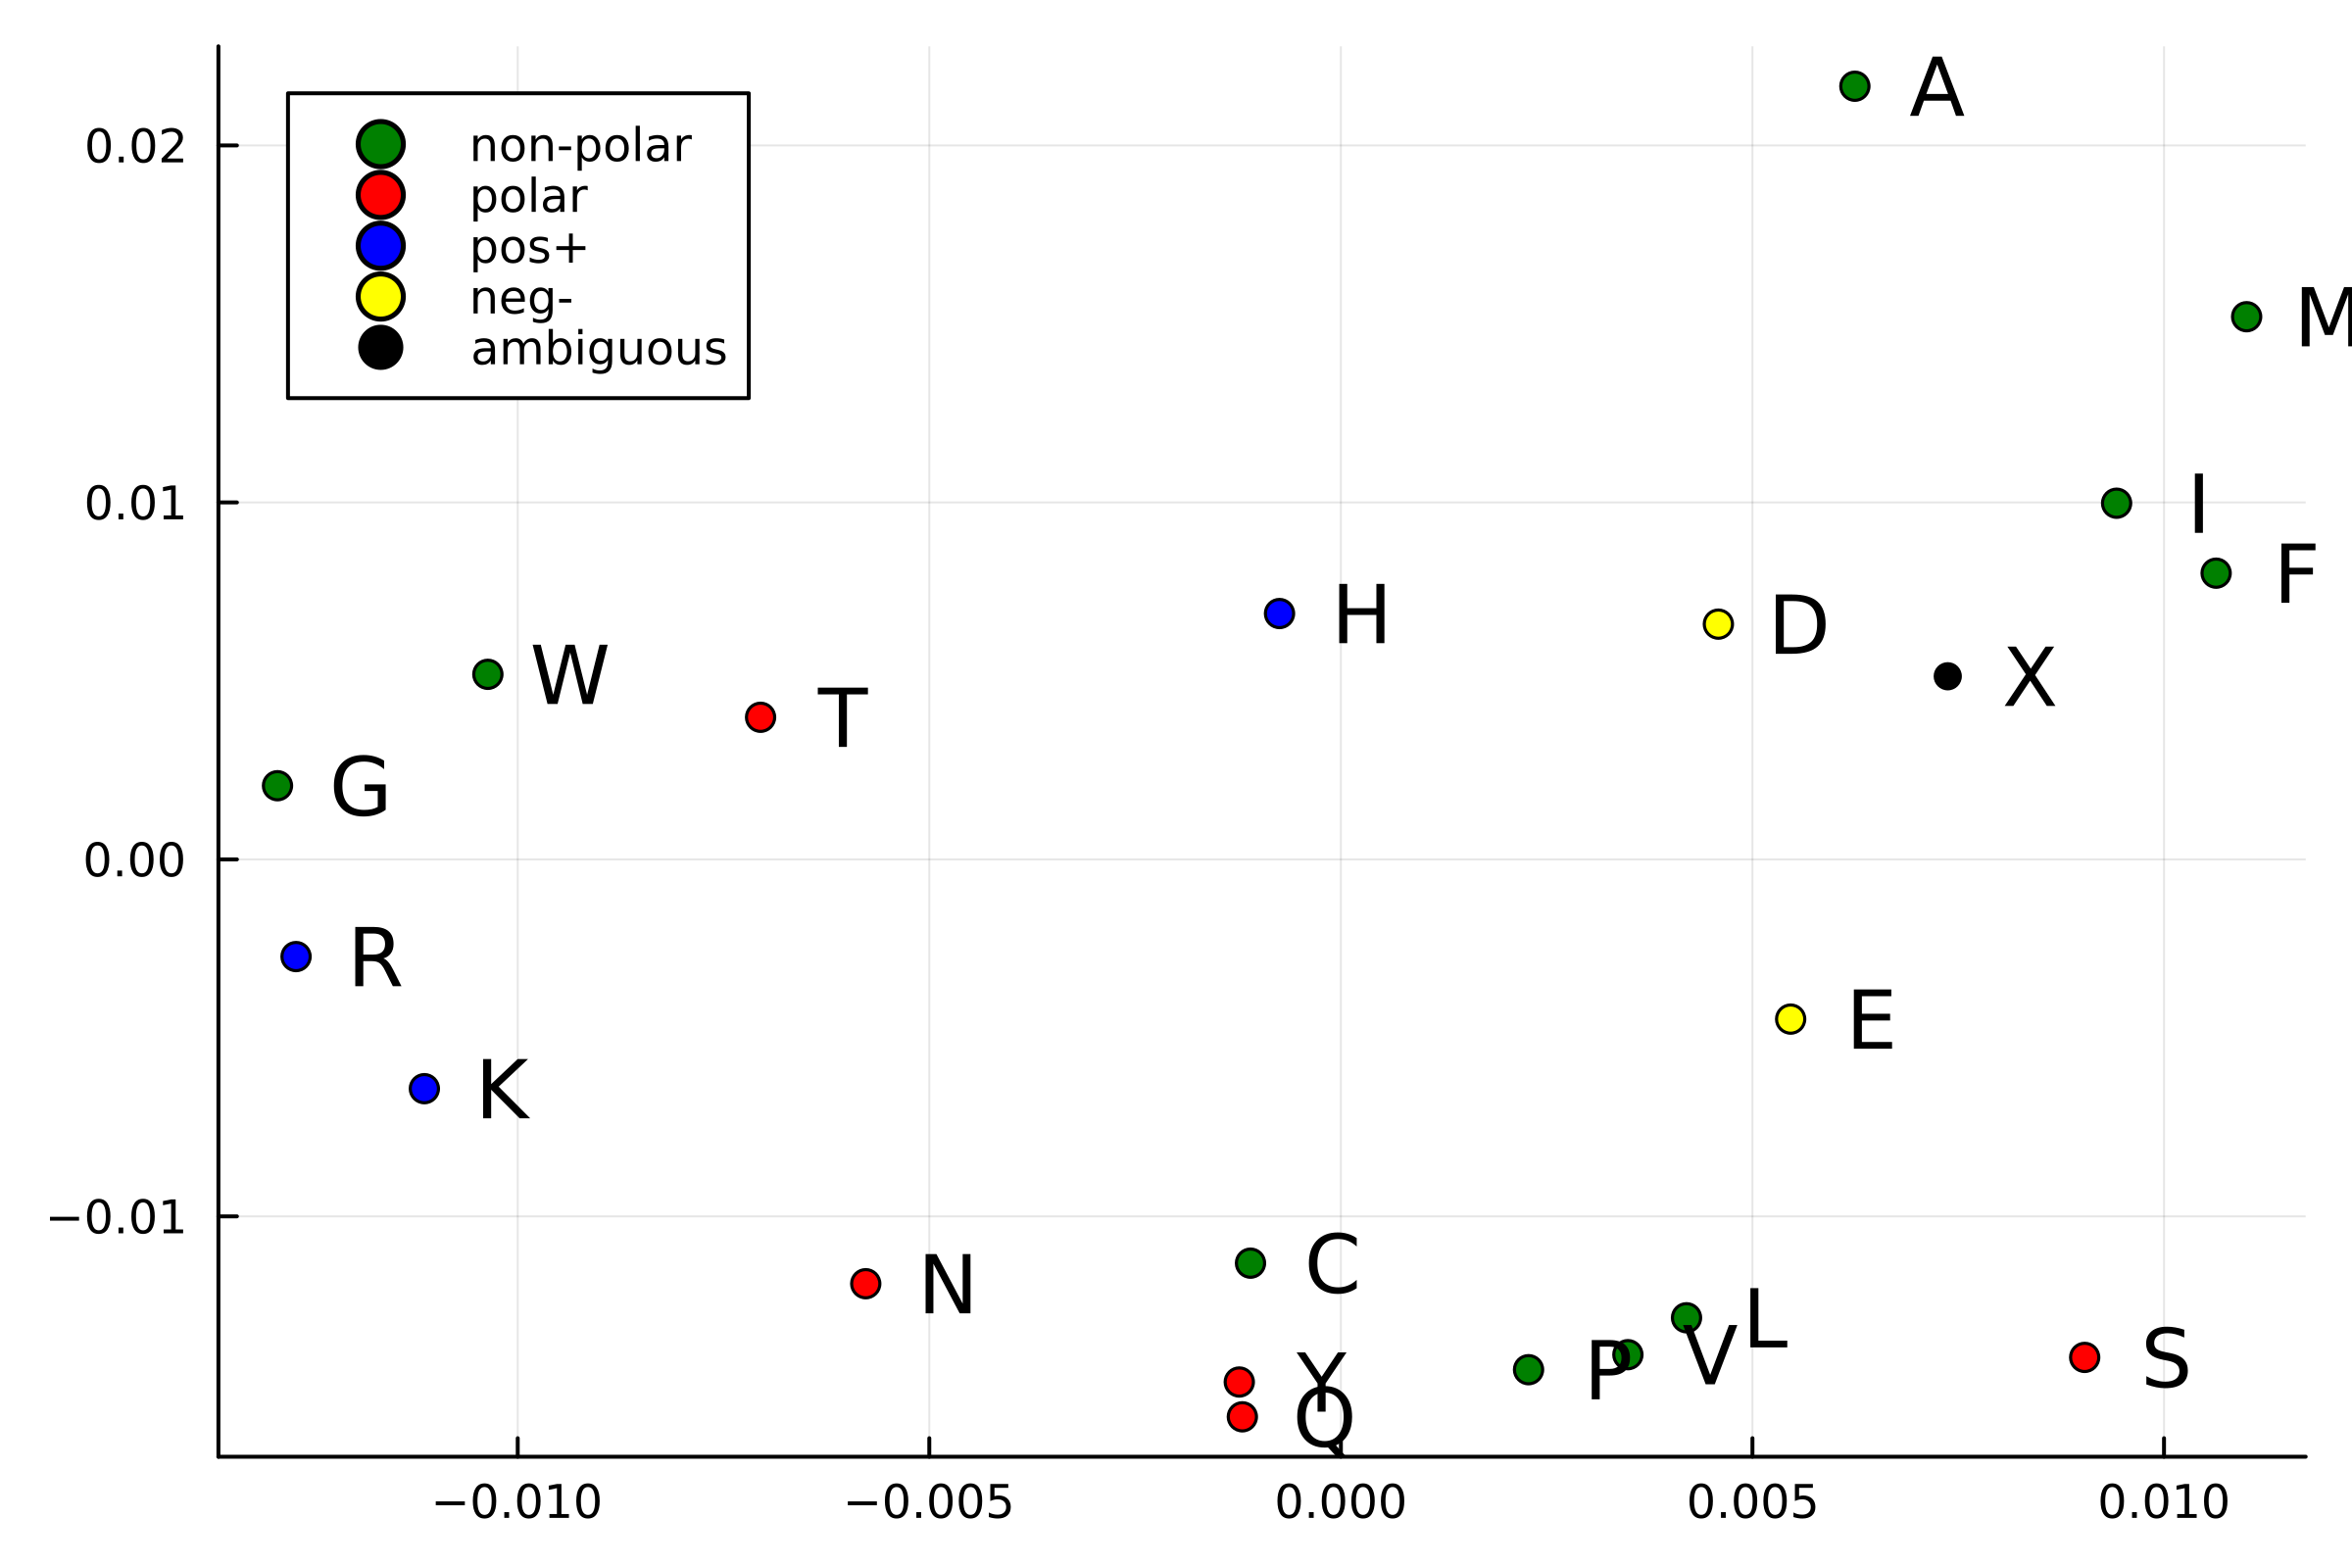
\includegraphics[width=\textwidth]{esm_emb_HDVreal}
    \caption{Real-value projected ESM-2 embeddings.}\label{fig:AAesmreal}
\end{subfigure}
\end{minipage}
\caption{Scatter plots of the first two principal components of ESM-2 embeddings for amino acids. (a) Unaltered 1024-dimensional ESM-2 embeddings, accounting for roughly 79 \% of the total variance. (b) ESM-2 embeddings projected into hyperdimensionality, accounting for roughly 22 \% of the total variance. (c) real-valued projected ESM-2 embeddings, accounting for roughly 28.5 \%. In all subfigures, amino acids are annotated and colored based on their chemical property of polarity.}
\end{figure}

\subsection{Real-valued projected ESM-2 embeddings}
The PCA of the real-valued projected ESM-2 vectors, as seen in Figure~\ref{fig:AAesmreal}, appears to capture a greater proportion of the variance compared to their binary counterparts. This increased detected variance is likely attributed to the reduction in data loss that occurs when avoiding the rounding off of values. The effectiveness of these real-valued projected ESM-2 vectors in various tasks will be further investigated and evaluated in subsequent analyses.

\subsection{Enforcing similarities using genetic algorthims}
The outcomes of employing a genetic algorithm to infer our target distances can be found in the tables located in Section~\ref{app:chp3} of the appendices. These are visually presented as heatmaps in Figure~\ref{fig:ga}. Taking into account that two random hyperdimensional vectors would be quasi-orthogonal just by stochasticity, their Hamming distances would be close to 0.5. Hence, one could see that despite our efforts, our obtained distances remain significantly different from the desired values and still indicate quasi-orthogonality, which led us to discontinue further exploration of these vectors. This discrepancy is likely attributable to the vast search space associated with the problem, resulting in substantial computational time required to reach the target matrix. The optimization process ran for approximately 58 hours on a high-performance computing system. Unfortunately, utilizing a genetic algorithm does not appear to be a viable method for optimizing hyperdimensional vectors within an acceptable timeframe.

\begin{figure}[H]
    \centering
    \begin{minipage}[b]{.5\textwidth}
    \begin{subfigure}[b]{\textwidth}
        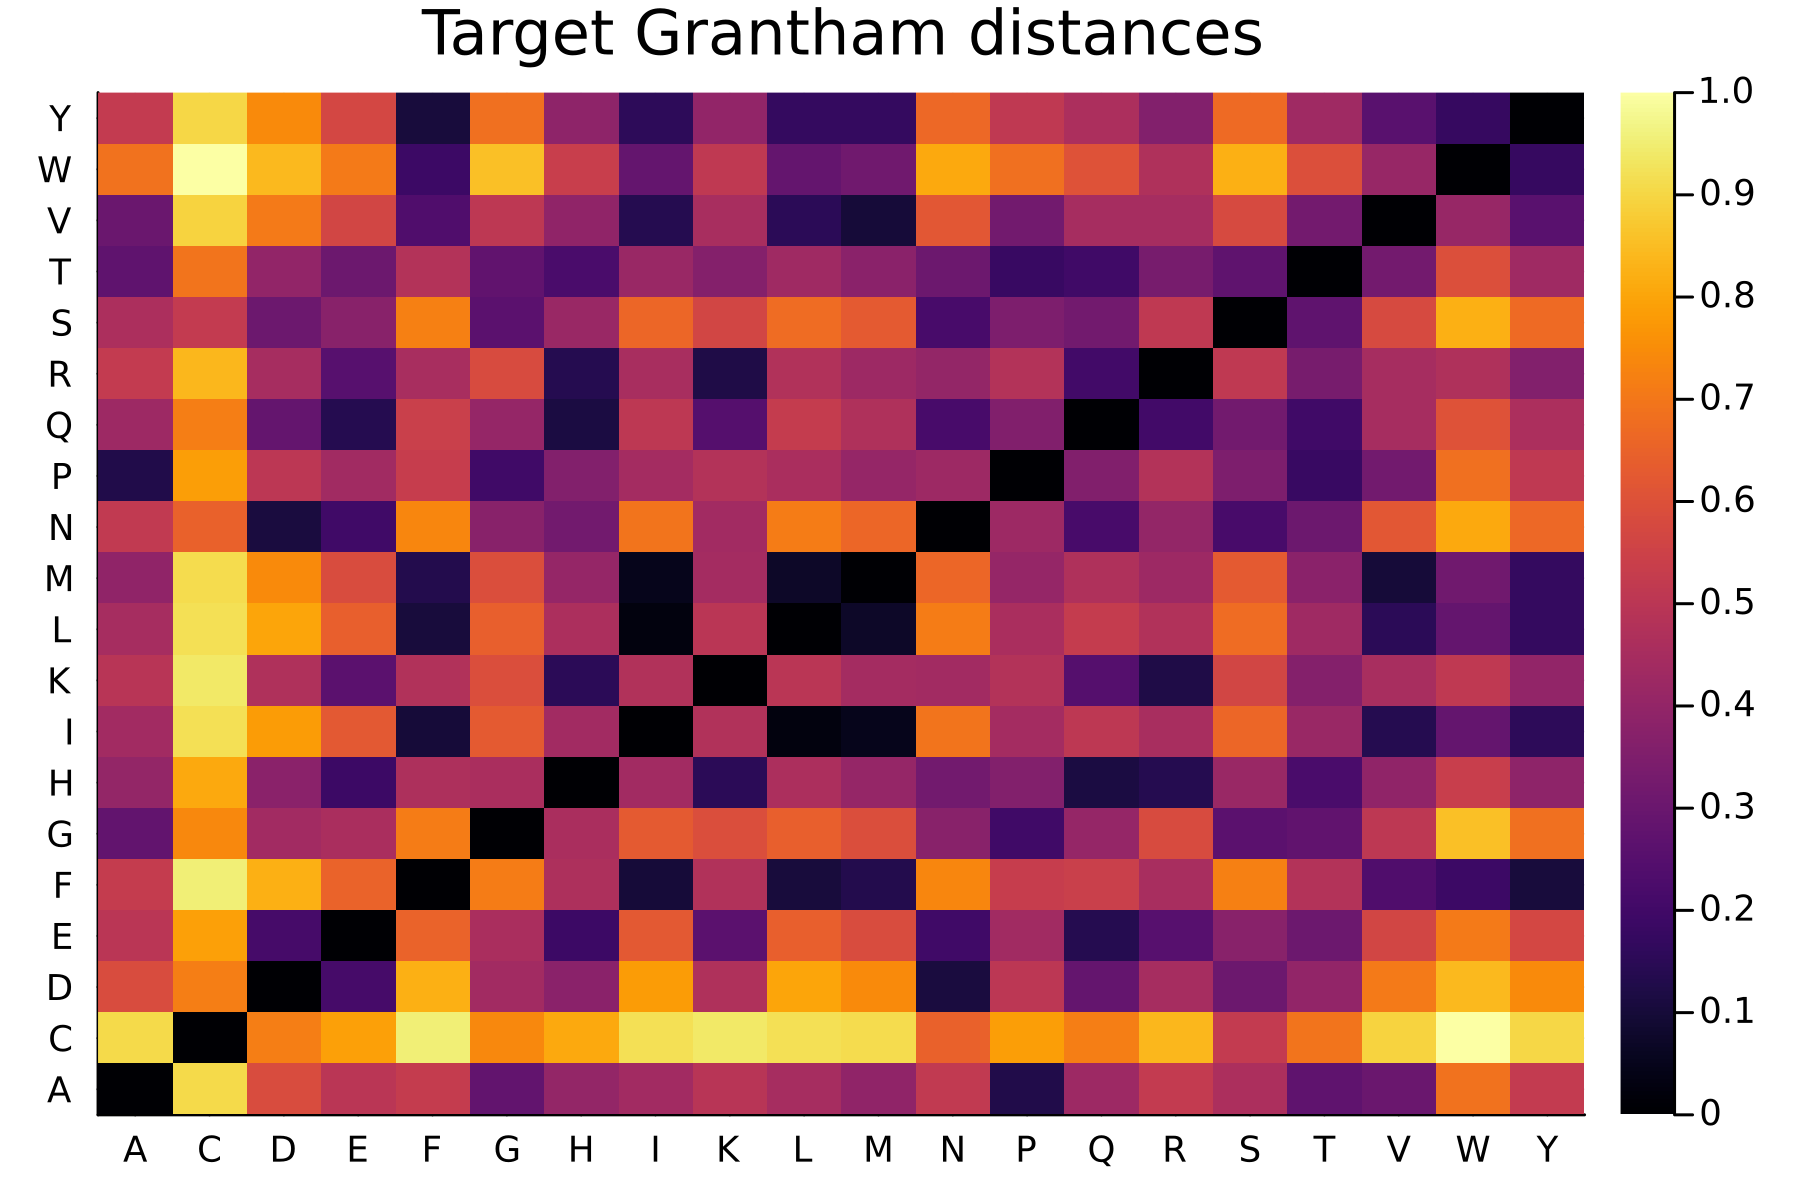
\includegraphics[width=\textwidth]{granttarget.png}
        \caption{Normalized Grantham's distance matrix.}
        \label{fig:grant}
    \end{subfigure}
\end{minipage}
\\
\centering
    \begin{minipage}[b]{.5\textwidth}
    \begin{subfigure}[b]{\textwidth}
        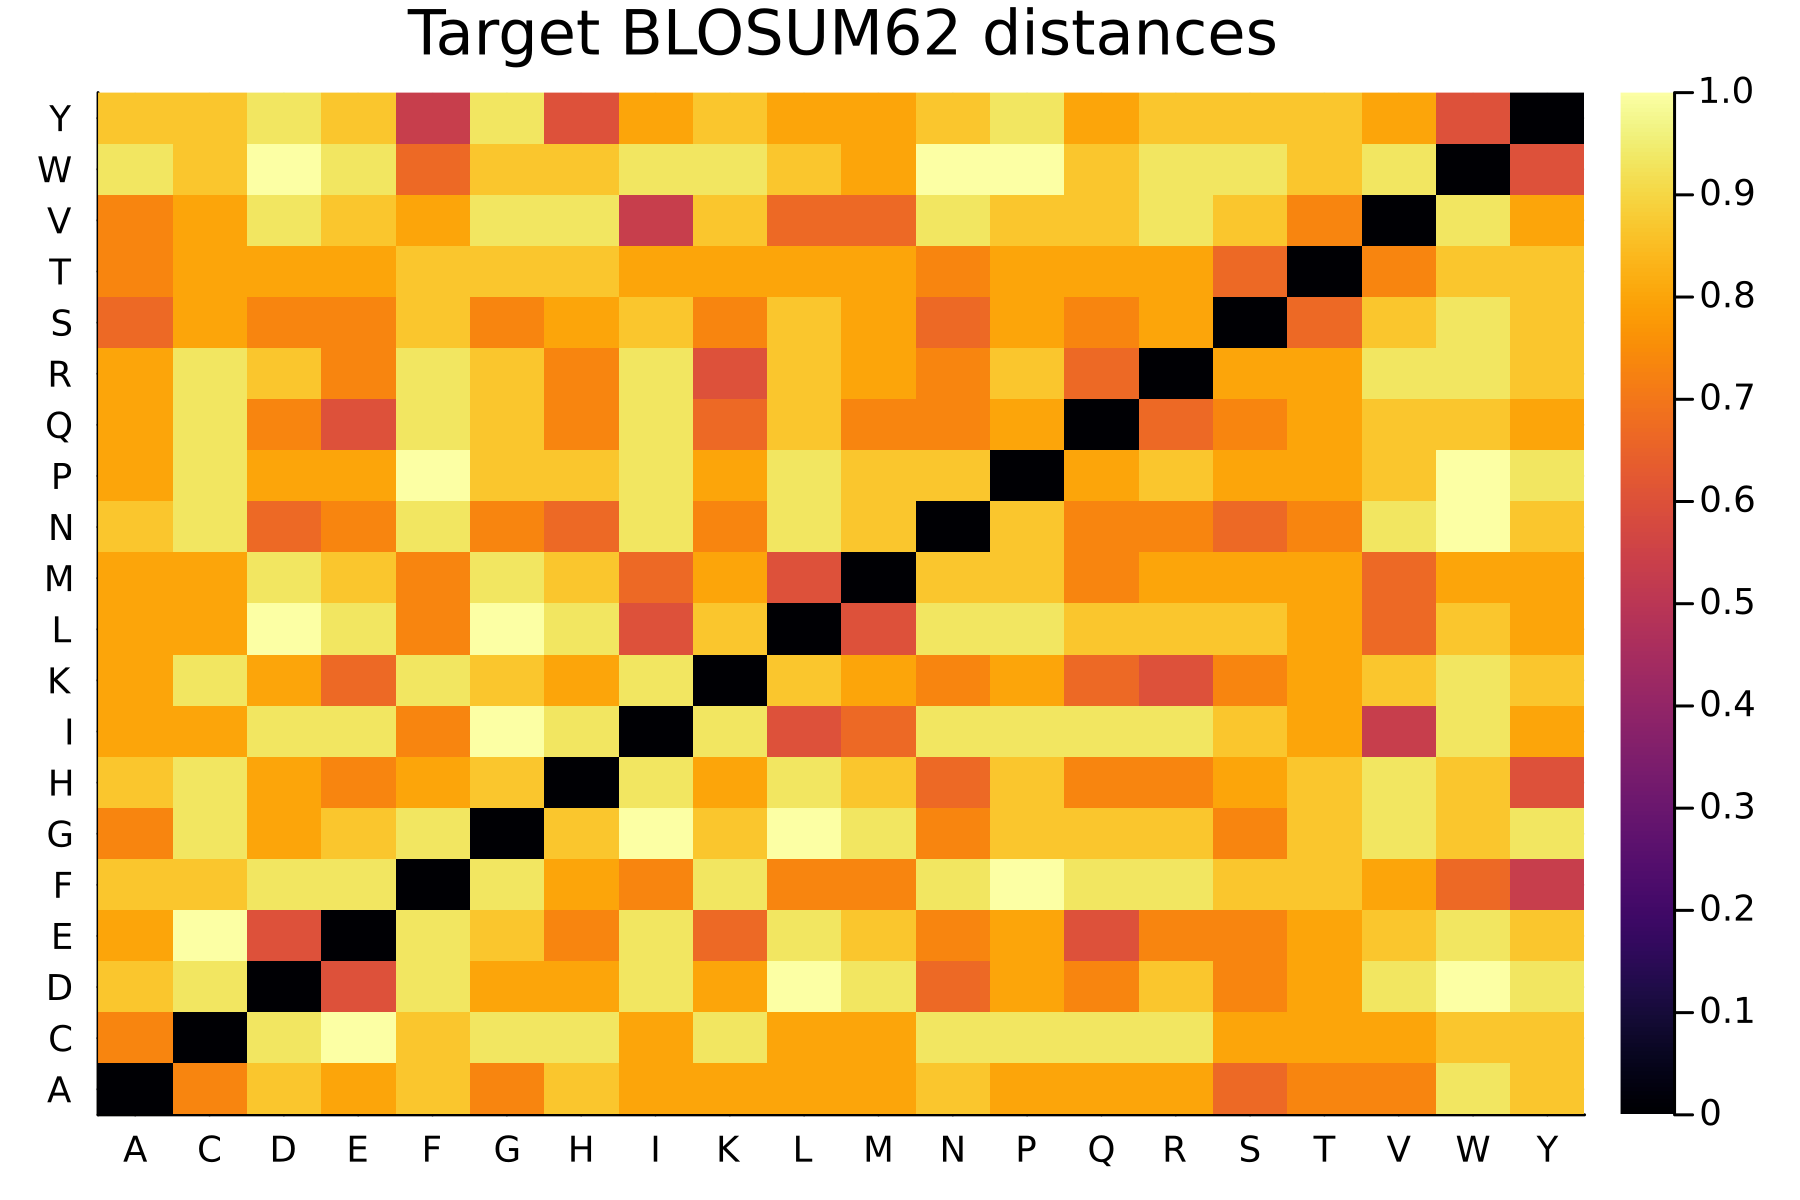
\includegraphics[width=\textwidth]{blosumtarget}
        \caption{Normalized amino acid distance matrix based on BLOSUM62.}
        \label{fig:blosum}
    \end{subfigure}
    \end{minipage}
\\
\centering
    \begin{minipage}[b]{.5\textwidth}
    \begin{subfigure}[b]{\textwidth}
        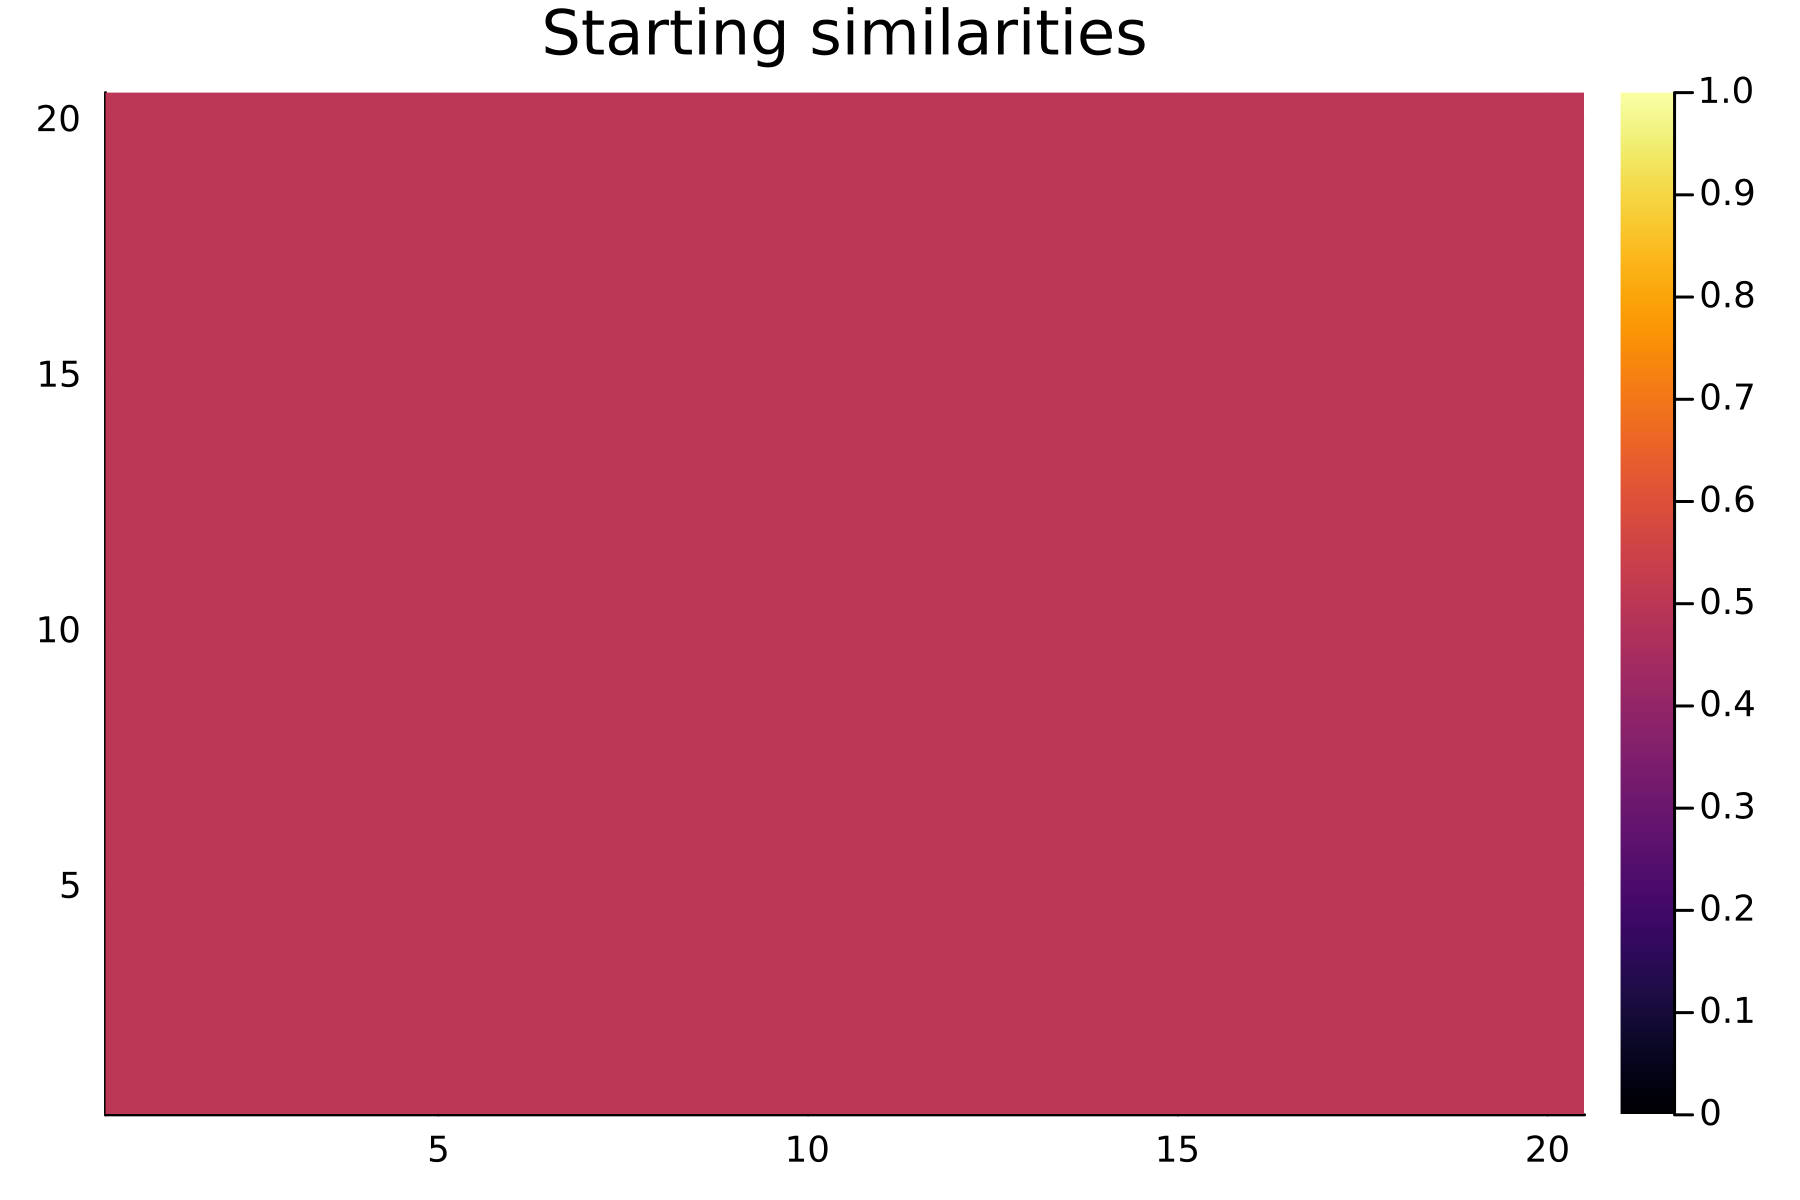
\includegraphics[width=\textwidth]{random}
        \caption{Achieved similarity matrix.}
        \label{fig:random}
    \end{subfigure}
    \end{minipage}
    \caption{Heatmap of the target pairwise amino acid distances, based on (a) Grantham's distance matrix (b) BLOSUM62 matrix and heatmap of (c) the achieved distances.}
    \label{fig:ga}
\end{figure}
\subsection{Contextualized neighborhood-encoding of amino acids}
Looking at the average neighborhood-encoded amino acids starting from ESM-2 embeddings and the human proteome (Figures \ref{fig:AAtr4} and \ref{fig:AAtr50}), the charged amino acids seem to be grouped vertically by PC 2, roughly dividing the polar and non-polar amino acids, albeit slightly more pronounced for $n = 50$. Also interesting, the very similar groupings in the PCA plots might indicate that the first four amino acids before and after a residue are the most crucial in encoding its information.

The PCA scatter plots generated from random vectors (Figures \ref{fig:AArtr4} and \ref{fig:AArtr50}) show slightly different results as compared to the ones starting from ESM embeddings. These PCAs also capture less variance, which may indicate that encoding biological information/similarities into the vectors beforehand might be useful. For $k = 4$, some typicalities are noticed such as the close grouping of the negatively charged amino acids (D and E) and the consistent triangular grouping of H, L and R. Nonetheless, for $k = 50$ with random vectors, we see results deviating from all the PCA scatter plots of other neighborhood-encoded amino acids, which could mean that a PCA is not able to capture the sparse information for this case or that these vectors might be oversaturated.

\begin{figure}[H]
    \centering
    \begin{subfigure}[b]{0.45\textwidth}
        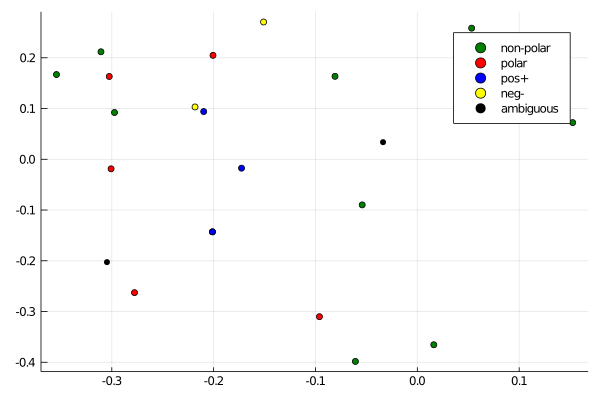
\includegraphics[width=\linewidth]{4tr_emb}
        \caption{$n = 4$ from projected ESM-2 embeddings, accounting for 21 \% of the total variance.}
        \label{fig:AAtr4}
    \end{subfigure}
    \hfill
    \begin{subfigure}[b]{0.45\textwidth}
        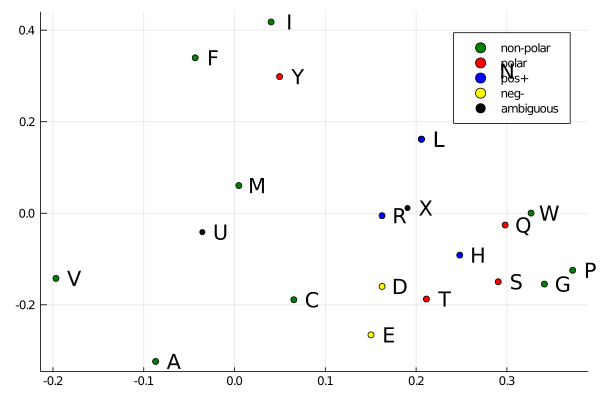
\includegraphics[width=\linewidth]{50tr_emb}
        \caption{$n = 50$ from projected ESM-2 embeddings, accounting for 21 \% of the total variance.}
        \label{fig:AAtr50}
    \end{subfigure}
    \vspace{10pt} % Add vertical space between rows
    \begin{subfigure}[b]{0.45\textwidth}
        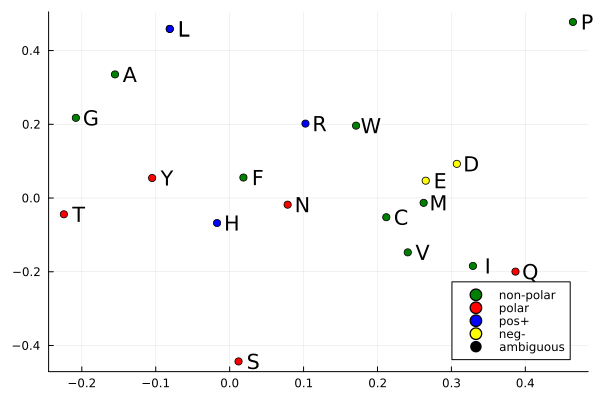
\includegraphics[width=\linewidth]{r4tr_emb}
        \caption{$n = 4$ from random vectors, accounting for 11 \% of the total variance.}
        \label{fig:AArtr4}
    \end{subfigure}
    \hfill
    \begin{subfigure}[b]{0.45\textwidth}
        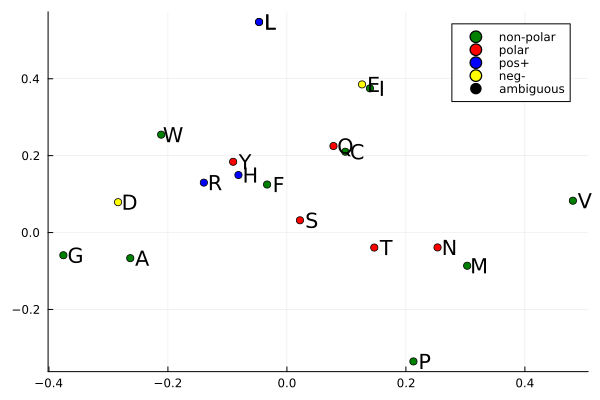
\includegraphics[width=\linewidth]{r50tr_emb}
        \caption{$n = 50$ from random vectors, accounting for 11 \% of the total variance.}
        \label{fig:AArtr50}
    \end{subfigure}
    \caption{Scatter plots of the first two principal components of the average amino acid HDVs with neighborhood-information of $n = 4$ and $n = 50$ encoded, learned from the human reference proteome. The top row represents encoded amino acids starting from projected ESM-2 embeddings, and the bottom row represents encoded amino acids starting from random hyperdimensional vectors. The amino acids are annotated and colored based on their chemical property of polarity.}\label{fig:bigfig}
\end{figure}

\section{Discussion}\label{sec:dis3}
As our research into genetic algorithms was unsuccessful for hyperdimensional vectors, future research could focus on other types of optimization algorithms such as simulated annealing~\cite{sa} etc.\ to generate optimized sets of hyperdimensional vectors in acceptable timeframes.

Rives \textit{et al.}~(2011) conducted experiments using their transformer model, ESM-1b~\cite{esm}, which paralleled our attempts at projecting the neighborhood-encoded vectors into fewer dimensions. Our results are comparable to theirs, but not as cleanly grouped, which is likely due to several factors. For instance, due to the intrinsic stochastic nature of hyperdimensional computing, it is prone to capture some amount of noise. On top of this, it is difficult for dimensionality-reduction methods such as PCA to accurately capture the intricacies of 10,000-dimensional vectors into two dimensions. UMAP projections were also made for the resulting vectors of the neighborhood-encoder method, shown in Appendix A, but these did not reveal any new information. Future work could focus on refining projection methods for hyperdimensional vectors or exploring alternative data reduction techniques that are able to accurately visualize hyperdimensional data. 

For the neighborhood-encoder method in particular, the amount of data we used is not comparable to what Rives \textit{et al.}~\cite{esm} used in their training model: our method learned from fewer than 21,000 sequences whilst their model was trained on 250 million sequences. They also included sequences originating from all recorded organisms in the UniProt database at that time whilst we confined ourselves to human sequences. Secondly, hyperdimensional vectors have a limited capacity, meaning long-range dependencies of a residue will saturate the hyperdimensional vector depending on the range. We can predict the angle between a bundled vector and a randomly selected vector from said bundle vector by $\Theta = \arccos({2k \choose k}/2^{2k})$ with $2k+1$ equal to the number of sequences in the class~\cite{sathdv}. This approximation is valid for bipolar/binary vectors in hyperdimensions $(\ge 10,000)$. This equation also suggests that an increase in dimensions will not influence the angle, so a 1,000,000-dimensional vector would not have more capacity than a 10,000-dimensional one. Evaluating this equation by considering random 1001 vectors in a bundled vector, so $k = 500$, results in an angle of $88.6^{\circ}$. This indicates that a vector has a limited capacity: the more vectors we bundle together, the closer the angle will be to $90^{\circ}$ and thus the more dissimilar the bundled vector becomes to its components. This results in the bundled vectors not being representative anymore of a given dataset. However, note that this equation assumes that the bundled vector is a bundle of purely random vectors, which is not the case for most of our embeddings; it only provides us with a rough idea about the bundling capacity of a hyperdimensional vector. As we would bundle amino acids or protein sequences with varying similarities, the bundling capacity could be different, warranting further research in this domain.

In the forthcoming two chapters, we will delve into practical case studies that draw upon the methodologies explored in this chapter, engaging with protein sequence datasets and executing predictive tasks therein. \mbox{Chapter 4} is focussed on exploring classification tasks employing protein sequence embeddings, wherein we will research the power of hyperdimensional computing, on its own or in combination with established machine learning methods. In Chapter 5, we shift our focus toward the classification tasks on amino acid vectors by using our neighborhood-encoder method to create contextualized embeddings of amino acids and neural networks to classify these.